\documentclass[oneside]{article}
\usepackage{fullpage}

\usepackage[pdftex]{graphicx}
\DeclareGraphicsExtensions{.png,.pdf}

\usepackage{hyperref}

% For including code into the document
\usepackage{verbatim}

% Tweak the default fonts a little
\renewcommand\rmdefault{bch}
\usepackage[small]{caption}
\usepackage[small]{titlesec}
\linespread{1.2} 

\title{Stat 640 - Data Mining Competition Final Report}
\author{Matthew Delhey \\ Frank Portman}
\date{\today}

\raggedbottom

\begin{document}
\maketitle 

\section{Introduction}
Our data mining competition constituted developing a recommender system to predict movie ratings for the MovieLens dataset. Since the Netflix prize, such recommender system have become a large area of academic research and have are also studied as matrix completion and collaborative filtering problems. The centerpiece to many proposed solutions--including the best performers in our competition--has been the matrix singular value decomposition, or SVD. Indeed, adaptions of the SVD for matrix completion were one of the main focuses of our own recommender. After the completion of the competition our team was able to significantly increase our submission to what would have been 18th place by utilizing superior parameter selection for matrix completion and blending its predictions with a k-nearest neighbors approach.

\section{Summary of Performance}
\begin{figure}[htpd]
  \centering
  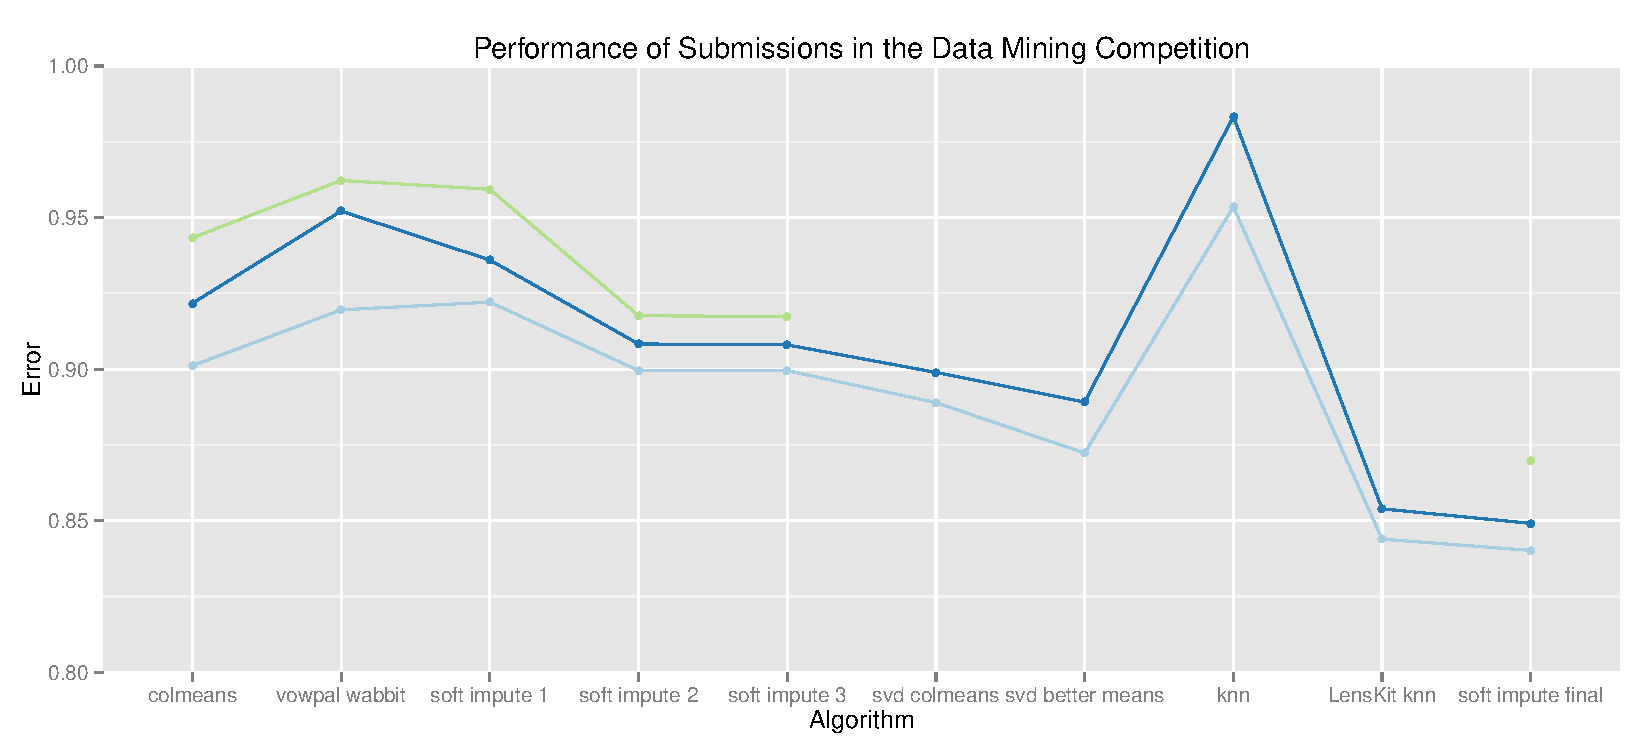
\includegraphics[width = 0.95\linewidth]{vis}
  \caption{Submissions are in chronological order along the x-axis. The top green line represents the leaderboard error, the middle dark blue line represents test error, and the light blue line represents test error. As we can see, not all methods were submitted to the leaderboard and our test error was lower than the leaderboard error.}
  \label{fig:one}
\end{figure}

Our best performing submission was a 60/40 blend of the Hastie and Mazumder implementation of the soft imputation algorithm and the LensKit k-nearest neighbors, which we will discuss in more detail in the ensemble section. We wish here to briefly discuss our other submissions. 

We began the competition by implementing the benchmark colmeans and the fast linear learner vowpal wabbit. We then divided our time by exploring SVD and nearest neighbor methods. As we know, the SVD factorization requires a complete matrix and is thus not directly applicable to our matrix completion problem. Our first solution was to begin with the colmeans predictions and proceed to find an appropriate low-rank approximation which could in turn be used to make new predictions. This resulted in methods \verb|soft impute 1| and \verb|soft impute 2| seen in Figure \ref{fig:one}, the latter starting first with a global mean. Further developments of the SVD were done through the use of the soft impute algorithm.

For k-nearest neighbors approaches, we began by running the naive algorithm on the entire dataset with a euclidean distance metric. As discussed in class, this method performed poorly for all values of $k$ and so we have only included one submission in our visualization. In order to facilitate exploration of k-nearest neighbors we later adopted the LensKit java framework. The framework is expansive and certainly worth exploring if one has some java background. There were two primary motivations to switching to such a framework over \verb|R| or \verb|MATLAB|: (i) speed, and (ii) preexisting software for easily producing predictions for our dataset. Indeed, the LensKit software has close ties to the GroupLens project that supplied our competition dataset. We will discuss our best k-nearest neighbors submission in more detail in the final section. 

As a small note regarding the post-processing of predictions, both of our primary models were capable of producing predictions outside of the rating domain $[1, 5]$. We clamped all predictions outside of these bounds before any kind of blending. 

Reflecting on the performance of our models in the competition, we were surprised at the RMSE one could achieve without delving into the auxiliary user and movie data. Our focus during the competition was entirely on the primary user-movie ratings matrix. Intuitively, it seems reasonable that there might be some important relationships between these additional features and the rating response yet in our basic attempts at predicting these ratings we never found a strong enough signal to warrant more resource allocation. Nonetheless, we suspect that at least a slight decrease in prediction error is achievable with proper utilization of this auxiliary data.

\section{Cross-validation \& Base Learners}
Throughout the training of all of our base learners, we conducted parameter tuning, model selection, and model assessment using traditional, repeated cross-validation. Our general procedure was to perform internal model selection using 5-fold cross-validation and then 10-fold cross-validation for parameter tuning on a hold-out set. We used the root-mean-squared error as an obvious choice of model performance, and the mean cross-validated RMSE for model selection. We also recognize the possibility for using the variance of the cross-validated RMSE for model selection but did not find practical use for such specificity in our competition experience.

The downfall of this approach was a dramatic increase in the amount of time required to assess base learners. This was a particularly challenging problem given the large size of our dataset and the computationally intensive models we wanted to build. Indeed, we believe that if the competition had provided a much smaller dataset that our team would have been able to fit several more base learners. Let us now talk about the base learners we \textit{did} fit.

\begin{description}
    \item[vowpal wabbit] Vowpal wabbit a speedy linear learner developed out of Yahoo Research and Microsoft Research. While we did not end up developing proper parameter optimization for vowpal wabbit in our solutions due to its difficulty of use and time constraints, we find the project to be extremely interesting and perhaps a good fit for future exploration in related problems. Without appropriate parameters the learner resulted in suboptimal prediction RMSE performance. 
    \item[k-nearest neighbors] As we know from our experience in the competition and from discussion in class, naive application of \verb|knn| did not result in great performance. This is particularly interesting given the general success found by k-nearest neighbor approaches in many collaborative filtering problems. We found success using k-nearest neighbors by making two changes to the traditional method. The first was the blending of traditional row-based nearest neighbors with column-based nearest neighbors. In the LensKit framework, this is known as User (or UserUser) based collaborative filtering and Item (or ItemItem) based collaborative filtering, respectively. By selecting an optimal $k$ individually for both methods then blending of the results of the two, we were able to make much more accurate predictions compared to the standard k-nearest neighbors algorithm. The second and equally important change was the switch from euclidean distance to Hamming distance, which we found through cross-validation to be the most optimal of the easily available distance metrics. 

By making these and other small changes with the LensKit framework we were able to make k-nearest neighbors work rather well for our dataset. On the other hand, our implementation of \verb|knn| still did not seem to give the relative performance found in the Belkor methods for the Netflix prize. We believe that this is perhaps due to the smaller size of our dataset, giving \verb|knn| less data to learn from and thus less success for similar values of $k$. We particularly liked \verb|knn| for its interperateability and flexibility. 
    \item[singular value decomposition] Since the Netflix prize, the SVD has become nearly synonymous with matrix factorization, recommendation systems, and collaborative filtering. But as we have stated early, the SVD is only defined for complete matrices and thus as a matrix factorization alone it cannot solve the problem at hand. To overcome this, we used a ``soft start'' for the SVD by first attempting to fill in all missing values with some simple measure, and then making new predictions using the low rank approximation, as outlined in the previous section. The models of this form that we attempted to learn on the dataset had moderate performance but would not by any means win us the competition. We concluded from our results that we needed to implement a more sophisticated method for using the SVD to generate a low rank approximation to our ratings matrix.
    \item[softImpute] While softImpute is perhaps not a base learner it certainly was the best performing stand alone algorithm we ran on our dataset. The soft impute algorithm performs matrix completion using the nuclear norm regularization discussed in class. Rather than a simple two step process used for matrix completion in the previous learner, this soft impute algorithm iteratively fits SVDs to fill in the missing values. Additionally, this singular value decomposition differs from the method implemented previously because it is a soft-thresholding as opposed to the hard-thresholding used to achieve the exact low rank approximation of a complete matrix. 

Fitting this model in a computational feasible manner involved choosing appropriate rank max and lambda as well as a convergence threshold. We found choosing a low rank to be important for avoiding overfitting. Lambda represents the familiar regularization parameter for the nuclear norm. Finding the optimal lambda value through cross-validation was not an easy task: the fitting of the model required significant computational time. Finally, the convergence threshold measures the relative change in the Forbenius norm between any two successive estimates. Lowering the convergence threshold did little to aid in predictions and only increased the computational challenges in our experiences. 

Overall we found this method to be a great base learner and used it to constitute the majority of our recommendation system. The project is written entirely in R and it's source code is available on the CRAN archives. Our team found it particularly interesting to look at the implementation of the library to understand more clearly how the predictions were being generated. Given more time for the competition we believe our predictions could be further improved by augmenting the package source code with other ideas found in the recent literature on recommendation systems. We saw in the Netflix prize the ensembling of many different SVD-esque algorithms, so we hypothesize that such an adaptation could be successfully blended with our current predictions.
\end{description}

Looking at all of our base learners, we be live we successfully explored many of the possibilities of the SVD and k-nearest neighbors. At the same time, we understand that one can never train too many base learners in a data mining competition. Given additional resources, we would spend more time training base learners. One particular advantage of doing so would be the ability to expand our ensembling system. As a rule of thumb, ensembles of base learners result in the best prediction errors, as we discuss regarding the ensembling of our two most sophisticated base learners: soft impute and k-nearest neighbors. 

\section{Ensemble \& Model}

\begin{figure}[htpd]
  \centering
  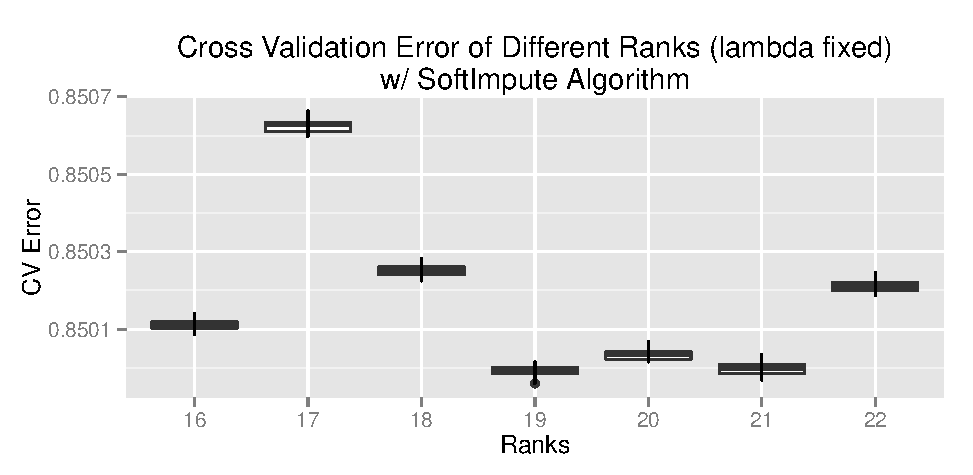
\includegraphics[width = 0.95\linewidth]{cvsi}
  \caption{Note that the stability of the cross-validation errors is due to the fact that these are \textit{repeated} cross-validation errors, i.e. are the average of 10-times repeated 10-CV error. The distribution of the CV-errors stays relative constant from rank to rank.}
  \label{fig:two}
\end{figure}

As stated previously, our best performing recommendation system was a 60/40 blend between the predictions of the soft impute algorithm and those from the LensKit k-nearest-neighbors. In Figure \ref{fig:two} we demonstrate our method for determning the best rank of the ratings matrix. We use much the same scheme for choosing the best $k$ in our neighbors model. 

The idea for building our ensemble came from the research literature which suggested that the error from these two types of models is sufficiently distinct that their mean might lead to better prediction error. Instead of doing a 50/50 split, we applied the our belief that our soft impute model was suprior to the nearest neighbor model due to its lower cross-validation error and decided with upon a 60/40 split. An easy improvement to our recommendation system would to be to perform cross-validation in order to determine the best linear split of the predictions.

In the future, we would spend more time and resources on developing a more sophisticated ensemble. If we were to train more viable base learners, it would be a more meaningful task to attempt to produce more complex ensembles utalizing the methods discussed in class such as boosting, bagging, and randomization.  

\section{Further Discussion}

\subsection{Innovation}
The innovation of our recommender system comes not from its theoretical properties but from its unique melding of various, disconnected software. We openly admit that the algorithms we used for our base learners were not novel and we instead place emphasis on our weaving together of open-source implementations and methods.

We also expiremented with the warm starts for our SVD. The use of colmeans and global means were obvious places to start, but we also explored using the auxilary data as well as considering ratios of rowmeans and colmeans. Ultimately we found a linear combination of row and colmeans to be the best, but was signifcantly outperformed by our other methods. 

\subsection{Literature}
We believe our recommender system is characterstic of the most popular methods in the relevant literature, especially that regarding the Netflix prize. Due to the similairties between the two data mining competitions, study of the Netflix prize and its best contestents greatly aided in the development of our own solutions as well as our general understanding of the problem. 

On the SVD side of our recommender, we are certainly within the domain of ongoing research. The Netflix prize and its subsequent research has shown the SVD to be incredibly useful tool for matrix completition. The same holds true for the \verb|knn| side of our recommender, which has a history of popular usage for similar systems. One of the benefits of neighbor-based approaches is their generous interpretations for both the data analyst and the end user. For example, ItemItem collaberative filtering allows the recommendation system to justify its recommendations to the users by telling the user the items from which it is making its new recommendation. Overall, we found the literature to be particularly engaging on the topic and certainly plentiful for the aforemented Netflix competition.

\section{Lessons and Remarks}
As our team's first foray into data mining, the competition was certainly a learning experience. We saw two primary catagories of lessons to be learned from the competition. The first concerned the theortical aspects of exploring the literature of recommender systems and their complexity. This catagory of lessons tended to coincide more with the general class lectures and the statistics within data mining. 

The other catagory of lessons was highly practical and represented more of the programming examples. Indeed, we found the assignment to be fundamentally a programming one involving the piecing together of preexisting software. In this vain, we were suprisied by the importance of computational considerations. Even seemingly simple problems such as calcuating the correlation matrix for our dataset became difficult on commodity hardware. The sucesfull use of DAVinCI was vital when doing our large cross-validation folds over the softImpute library in R. We were able to perform our LensKit computations on local machines due to its faster performance. These problems added a technical dimention to the competition that parallels the deepening technical problems facing practical data analysis on today's largescale datasets and thus the competition satsfying in its pragmatism. 

\section*{Appendix: Team Contributions}
For our team, the data mining competition was an extremely collaborative effort. While there were distinct allocations and distributions of work, they did not necessarily indicate that the other team member was not also additionally involved. At a high level, much of the SVD code was done by Frank while the k-nearest neighbors and LensKit code was done by Matt. The final blending of the models and the final report were a collaborative effort. 


\begin{thebibliography}{1}
  \bibitem{}Bell, R. M., Koren, Y., \& Volinsky, C. (2007). The BellKor solution to the Netflix prize. KorBell Team’s Report to Netflix.

  \bibitem{}Ekstrand, Ludwig, Konstan, Riedl, (2011): Rethinking the Recommender Research Ecosystem: Reproducibility, Openness, and LensKit. The Fifth ACM Conference on Recommender Systems, Proceedings of the Fifth ACM Conference on Recommender Systems Association of Computing Machinery Association of Computing Machinery, Chicago, IL, 2011.

  \bibitem{}Langford, J., Li, L., \& Strehl, A. (2007). Vowpal wabbit online learning project.

  \bibitem{}R Core Team (2013). R: A language and environment for statistical
  computing. R Foundation for Statistical Computing, Vienna, Austria.
  URL http://www.R-project.org/.

  \bibitem{}Trevor Hastie and Rahul Mazumder (2013). softImpute: matrix
  completion via iterative soft-thresholded svd. R package version 1.0.
  http://CRAN.R-project.org/package=softImpute

  \bibitem{}This work was supported in part by the Data Analysis and Visualization Cyberinfrastructure funded by NSF under grant OCI-0959097.

\end{thebibliography}

\end{document}
